\documentclass{standalone}
\usepackage{tikz}
\usepackage{hsbcommon}
%% Show/hide steps for standalone work — edit this line:
\makeatletter\AtBeginDocument{\@buildstepset{1,2,3,4}}\makeatother
\begin{document}

    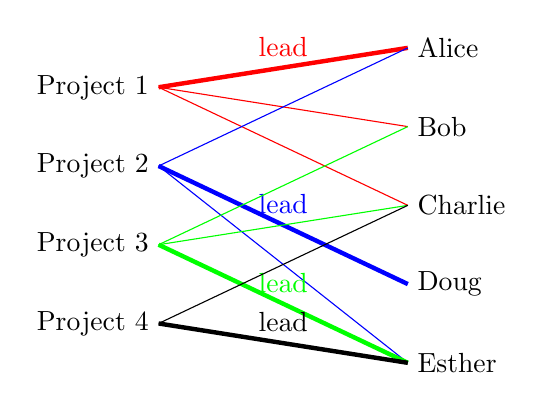
\begin{tikzpicture}
        \foreach [count=\i] \ii in {1,...,4}
            \node (p\i) at (0,-\i-0.5) {Project \i};
        \foreach [count=\i] \ii in {Alice, Bob, Charlie, Doug, Esther}
            \node[anchor=west] (\ii) at (4,-\i) {\ii};

    \ifstep{1}{
        \begin{scope}[red]
            \draw[ultra thick] (p1.east) -- node[midway,above] {lead} (Alice.west);
            \draw[] (p1.east) -- (Bob.west);
            \draw[] (p1.east) -- (Charlie.west);
            
        \end{scope}
    }
     \ifstep{2}{
        \begin{scope}[blue]
            \draw[] (p2.east) -- (Alice.west);
            \draw[ultra thick] (p2.east) -- node[midway,above] {lead} (Doug.west);
            \draw[] (p2.east) -- (Esther.west);
            
        \end{scope}
    }
    
     \ifstep{3}{
        \begin{scope}[green]
            \draw[] (p3.east) -- (Bob.west);
            \draw[] (p3.east) -- (Charlie.west);
            \draw[ultra thick] (p3.east) -- node[midway,above] {lead} (Esther.west);
        \end{scope}
    }
    
        \ifstep{4}{
        \begin{scope}[black]
            \draw[] (p4.east) -- (Charlie.west);
            \draw[ultra thick] (p4.east) -- node[midway,above] {lead} (Esther.west);

        \end{scope}
    }
    
        
        
        
        % \draw[color=black] (p4) -- (Esther);

    \end{tikzpicture}
\end{document}